\documentclass{report}
\usepackage[utf8]{inputenc}
\usepackage{graphicx}
\usepackage[portuguese]{babel}


\title{Principal Component Analysis - PCA}
\author{Julia Del Giudice e Sofia Iara}
\date{06 de Dezembro de 2022}

\begin{document}
\maketitle

\section{Dataset}
O dataset utilizado para a análise foi o Mobile Price Classification, que se trata de uma classificação de preços de celulares pelas suas especificações. Retirado do site Kaggle com 21 colunas e 2000 registros, as colunas são:
\begin{itemize}
\item battery power: energia total que a bateria possui. Medida em mAh.
\item blue: Se tem bluetooth ou não.
\item clock speed: Velocidade da execução micro-processador.
\item dual sim: Se suporta dois chip ou não.
\item fc: Os Mega Pixels da câmera frontal.
\item four g: Se suporta 4G.
\item int memory: Capacidade da memória interna em GB.
\item m dep: Especificação da profundidade do celular em cm.
\item mobile wt: Peso do celular.
\item n cores: Números de núcleos que o processador possui.
\item pc: Os Mega Pixels da câmera principal traseira.
\item px height: Altura da resolução da tela.
\item px width: Largura da resolução da tela.
\item ram: Capacidade da memória ram em MB.
\item sc h: Altura da tela do celular em cm.
\item sc w: Largura da tela do celular em cm.
\item talk time: Tempo de uma carga da bateria enquanto você consome.
\item three g: Se suporta 3G.
\item touch screen: Se suporta toque na tela.
\item wifi: Se suporta wifi.
\item price range: A classificação do preço, sendo 0 -> custo baixo; 1 -> custo médio; 2 -> custo alto; 3 -> custo muito alto.
\end{itemize}

\section{Matriz de Covariância do Dataset}
O primeiro passo que fizémos foi separar a coluna price range, que será nosso target, do dataset, para então calcular sua matriz de covariância:

\begin{figure}[htbp]
\caption{Primeiro Código}
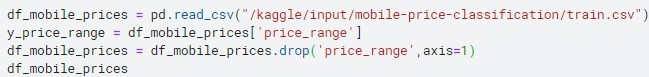
\includegraphics[width=12cm]
{figures/primeiro_codigo.jpg}
\label{figura com o primeiro código que foi feito}
\end{figure}

\begin{figure}[htbp]
\centering
\caption{Código da Matriz de Covariância}
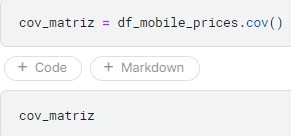
\includegraphics[width=6cm]
{figures/cod_matriz.jpg}
\label{figura com o código da matriz de covariância}
\end{figure}

\begin{figure}[htbp]
\centering
\caption{Matriz de Covariância}
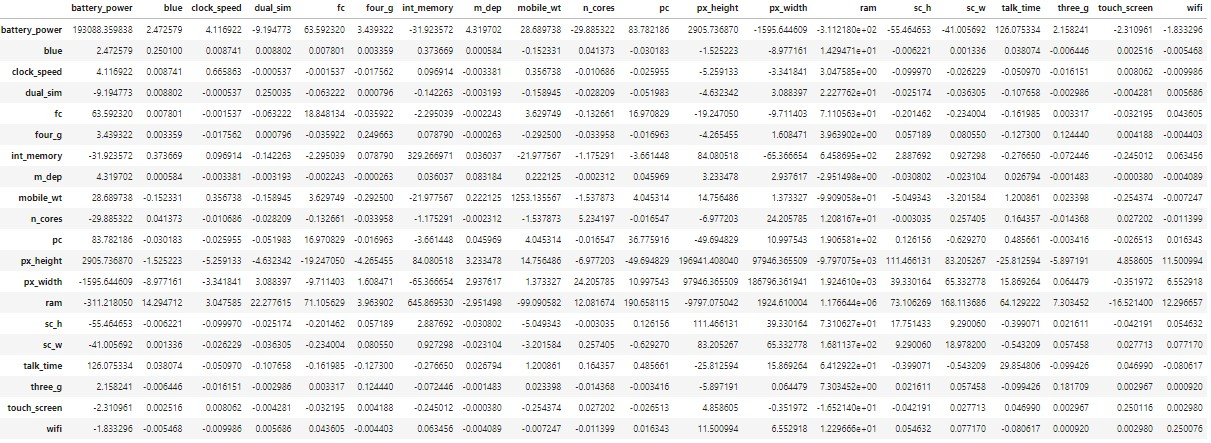
\includegraphics[width=13cm]
{figures/matriz_cov.jpg}
\label{figura com a matriz de covariância}
\end{figure}

\section{Calculando os Autovalores e Autovetores}
O terceiro passo foi calcular tanto os autovalores quanto os autovetores:

\begin{figure}[htbp]
\centering
\caption{Código para o Cálculo dos Autovalores e Autovetores}
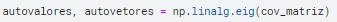
\includegraphics[width=12cm]
{figures/cod_autos.jpg}
\label{figura com o código dos autovalores e autovetores}
\end{figure}

\begin{figure}[htbp]
\centering
\caption{Autovalores do Dataset}
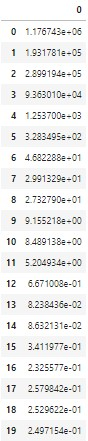
\includegraphics[width=2cm, height=4cm]{figures/autovalores.jpg}
\label{figura com os autovalores}
\end{figure}

\begin{figure}[htbp]
\centering
\caption{Autovetores do Dataset}
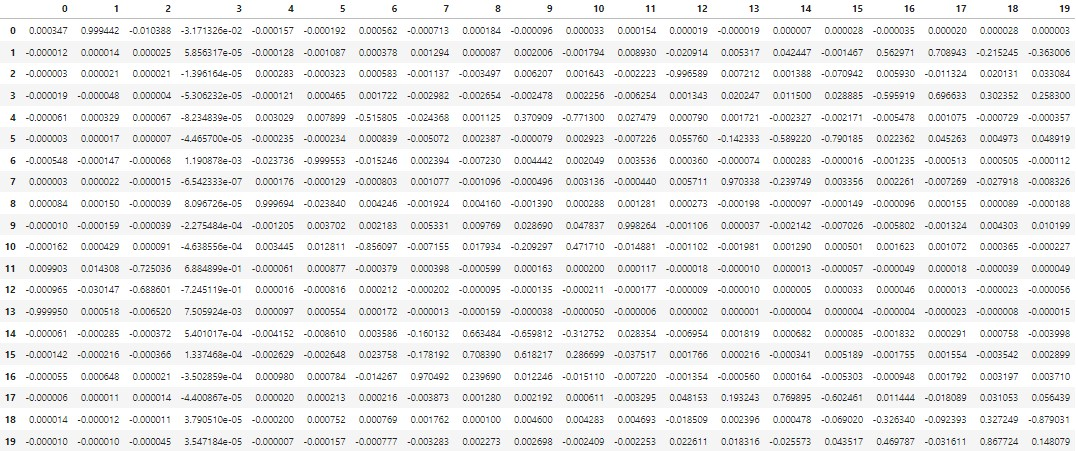
\includegraphics[width=12cm]{figures/autovetores.jpg}
\label{figura com os autovetores}
\end{figure}

\section{Selecionando os Dois Maiores Autovalores}
O quarto passo foi ordenar os autovalores e autovetores do maior para o menor e calcular a variância explicada e a variância explicada cumulativa que seriam o quanto cada componente (autovetores) está representando a variabilidade do dataset.

\begin{figure}[htbp]
\centering
\caption{Código dos Autovalores e Autovetores e da Variância Explicada}
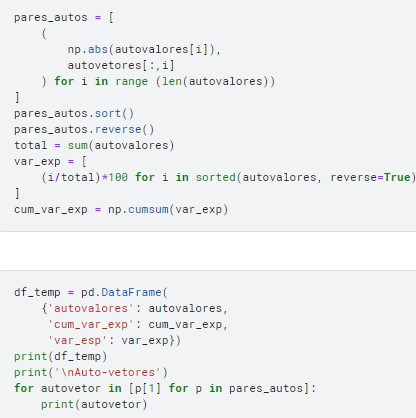
\includegraphics[width=6cm]{figures/cod_var_exp.jpg}
\label{figura com o código dos autovalores e autovetores e da variância explicada}
\end{figure}

\begin{figure}[htbp]
\centering
\caption{Autovalores (Sendo grifado os dois maiores) e Autovetores e da Variância Explicada}
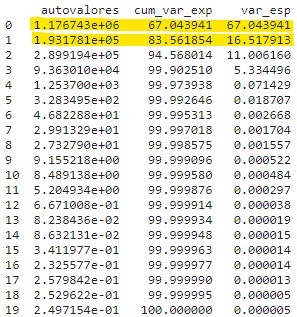
\includegraphics[width=6cm]{figures/maiores_autovalores.jpg}
\label{figura com os autovalores (grifandos os dois maiores) e autovetores e da variância explicada}
\\Como é possível observar, com os dois maiores autovalores temos variância explicada cumulativa de 83.56\%.
\end{figure}

\section{Colunas Referentes aos Autovalores}
Para partir para a plotagem das colunas correspondentes aos dois maiores autovalores, foi preciso transformar o dataset com os autovalores mencionados e adicionar a coluna price range neste dataset transformado.

\begin{figure}[htbp]
\centering
\caption{Transformação para o Dataset}
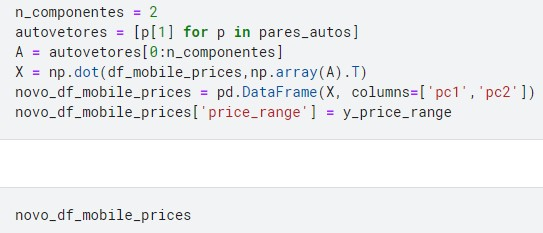
\includegraphics[width=6cm]{figures/cod_mudanca_p_dataset.jpg}
\label{figura com o código da transformação para o dataset}
\end{figure}

\begin{figure}[htbp]
\centering
\caption{Dataset com as Colunas Correspondentes}
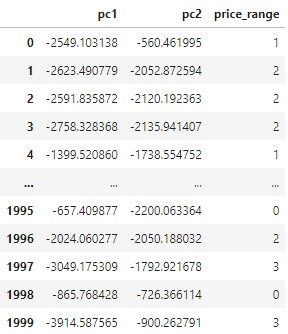
\includegraphics[width=6cm]{figures/dataset_transformado.jpg}
\label{figura com o dataset transformado}
\end{figure}

\section{Plotagem das Colunas Correspondentes dos maiores Autovalores em Relação ao Dataset}
O último passo é trazer esse dataset transformado em gráfico.

\begin{figure}[htbp]
\centering
\caption{Código com a Plotagem para o Gráfico}
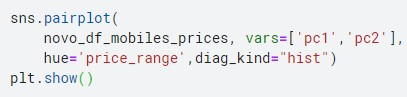
\includegraphics[width=10cm]{figures/cod_plot.jpg}
\label{figura com o código da plotagem do gráfico}
\end{figure}

\begin{figure}[htbp]
\centering
\caption{Gráfico das Colunas Referentes aos Dois Maiores Autovalores}
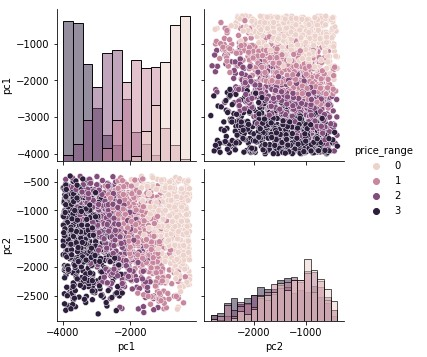
\includegraphics[width=12cm]{figures/plot_novo_dataset.jpg}
\label{figura com o gráfico das colunas referentes aos dois maiores autovalores}
\end{figure}

\end{document}


